\documentclass[12pt,a4paper]{article}
 
\usepackage{float}
%für feststellen der figures und tables [H] dranschreiben
\usepackage{units}
%wird so benutzt: 
%\unit[value/Zahl]{dimension/Einheit} oder 
%\unitfrac[value/Zahl]{dimension/Einheit num/Zähler}{dimension/Einheit denum/Nenner} oder
%\nicefrac[fontcommand/Schriftart]{dimension/Einheit num/Zähler}{dimension/Einheit denum/Nenner}

\usepackage{caption}
\usepackage{subcaption}

\usepackage[left=2cm,right=2cm,top=2cm,bottom=2cm]{geometry}
\usepackage[utf8]{inputenc}
\usepackage[T1]{fontenc}
\usepackage{lmodern}
\usepackage[ngerman]{babel}
\usepackage{amsmath}
\usepackage{graphicx}
\usepackage{framed} 	%Verwenden um Text einzurahmen
 
\title{Regelschaltungen}
\author{Frederik Strothmann, Henrik Jürgens}
\date{\today}
%niemals zwei überschriften direkt übereinander schreiben, also immer mindestens in einem satz was sinnvolles unter jede überschrift schreiben (bei den versuchen z.B. das versuchsziel) 
\begin{document}
%deckblatt erstellen.
\maketitle
\newpage
\tableofcontents
\newpage
\section{Einleitung}
%einleitung zu dem experiment.
%auf die einstellungen, die vor dem versuch gemacht werden, eingehen oder auf eine anleitung dazu verweisen
%es soll immer erwähnt werden um was es in dem Versuch geht und wie das relisiert werden soll
%---------------------------------------------------------------------------------------------
%hinter der einleitung kann der allgemeine theoretische hintergrund in einer zusätzlichen section erklärt werden
%1-----------------------------------------------1

In diesem Versuch werden Regelschaltungen untersucht, dies finden in den meisten heutzutage erhältlichen Geräten Anwendung, z.B Computer und Autos. Es werden vier verschiedene Regelschaltungen untersucht, eine Zweiwegregelung, eine Zweiwegregelung mit Hysterese, eine Proportionalregelung und eine Proportionalregelung mit Integrator.


\section{Eichung des NTC-Sensors}
%kurz das ziel dieses versuchsteiles ansprechen, damit keine zwei überschriften direkt übereinander stehen!
%bei schwierigeren versuchen kann auch der theoretische hintergrund erläutert werden. (mit formeln, herleitungen und erklärungen)
Im ersten Versuchsteil soll der NTC-Sensor für die nachfolgenden Messungen geeicht werden. Der NTC-Sensor ist ein Widerstand, der Exponentiell von der Temperatur abhängt.

\subsection{Verwendete Geräte}
%(immer) eine skizze oder ein foto einfügen, die geräte/materialien !nummerieren! und z.b. eine legende dazu schreiben, besser wäre es das ganze in einem Fließtext gut zu beschreiben.
%falls am anfang des versuches nicht klar ist, was alles verwendet wird, wenn möglich erst am ende ein großes foto von den verwendeten materialien machen!\\.

Es werden ein NTC-Sensor, ein Kühlkörper, ein DMM, ein Heizwiderstand und ein Netzgerät verwendet.

\subsection{Verwendete Formeln}
%eine legende kann angefertigt werden, die selbstverständlichen buchstaben müssen nicht extra erklärt werden
%mit knappen erklärungen die !verwendeten! formeln, sowie die zugehörige fehlerrechnung einfügen
%2-----------------------------------------------2
%ab hier kann nochmal in einzelne versuchsteile unterteilt werden

Der Zusammenhang zwischen Widerstand und Temperatur ist durch Gleichung \ref{eqn:ntc} gegeben. R$_{25}$ ist der Widerstand bei 25$^\circ$C

\begin{align}
\text{R}_\text{NTC}(\text{T}) = \text{R}_{25} \text{exp}\left(-\text{B} \left(\frac{1}{\text{T}_{25}}-\frac{1}{\text{T}}\right)\right)
\label{eqn:ntc}
\end{align}

\subsection{Versuchsaufbau}
%skizze zum versuchsaufbau (oder foto) einfügen,   es muss erklärt werden wie das ganze funktioniert und welche speziellen einstellungen verwendet wurden (z.b. welche knöpfe an den geräten für die messung verdreht wurden)

1 ist der NTC, 2 ist der Kühlkörper und 3 der Heizwiderstand.

\begin{figure}[H] 
  \centering
    \includegraphics[ scale = 0.3]{Auf_1.png}
  	\caption[Aufbau zur Eichung des NTC]{Aufbau zur Eichung des NTC\footnotemark}
  \label{fig:auf_1}
\end{figure}
\footnotetext{Abbildungsteile entnommen von http://www.atlas.uni-wuppertal.de/$\sim$kind/ep7\_14.pdf am 06.12.2014}

\subsection{Versuchsdurchführung}
%erklären, !was! wir machen, !warum! wir das machen und mit welchem ziel
%(wichtig) präzize erklären, wie bei dem versuch vorgegangen und was gemacht wurde

Es wurde der Versuchsaufbau wie in Abbildung \ref{fig:auf_1} genommen und die grünen Kabel (der NTC) an ein DMM für die Widerstandsmessung angeschlossen. Danach wird der Heizwiderstand (das schwarze und das rote Kabel) an die 20V Gleichspannungsquelle des Netzgerätes angeschlossen. Dann wird das Digitalthermometer in die Bohrung des Hitzewiderstandes gesteckt und die Messung des Widerstandes in Abhängigkeit der Temperatur begonnen.

\subsection{Messergebnisse}
%die messwerte in !übersichtlichen! tabellen angegeben
%zu viele kleine tabellen in große tabellen überführen!
%zu große tabellen mit dem [scale]-befehl scalieren oder (falls zu lang) in zwei kleinere tabellen aufteilen
%(wichtig) vor !jeder! tabelle sagen, was gemessen wurde und wie die fehler gewählt wurden und ausreichend !erklären!, !warum! wir unsere fehler grade so gewählt haben

Der Fehler der Temperatur wurde mit dem Ablesefehler bestimmt, er beträgt \unit[0,1]{$^\circ$C}, da kein Fehler angeben war. Der Fehler des Widerstandes wurde aus dem Ablesefehler und dem angegebenen Fehler bestimmt, er beträgt \unit[60]{m$\Omega$} für alle Werte von \unit[21,4]{$^\circ$C} bis \unit[58]{$^\circ$C} und für die Werte von \unit[59]{$^\circ$C} bis \unit[69]{$^\circ$C} beträgt der Fehler \unit[6]{m$\Omega$}.

\begin{table}[htbp]
\centering
\begin{tabular}{||c|c||c|c||c|c||}

T/$^\circ$C & Widerstand/$\Omega$ & T/$^\circ$C & Widerstand/$\Omega$ & T/$^\circ$C & Widerstand/$\Omega$ \\ \hline
21,4 & 11,68 & 38 & 4,83 & 55 & 2,11 \\ 
22 & 11,34 & 39 & 4,58 & 56 & 2,04 \\ 
23 & 10,64 & 40 & 4,40 & 57 & 1,96 \\ 
24 & 10,02 & 41 & 4,20 & 58 & 1,88 \\ 
25 & 9,47 & 42 & 4,02 & 59 & 1,821 \\ 
26 & 9,00 & 43 & 3,85 & 60 & 1,734 \\ 
27 & 8,57 & 44 & 3,64 & 61 & 1,699 \\ 
28 & 8,09 & 45 & 3,45 & 62 & 1,602 \\ 
29 & 7,70 & 46 & 3,28 & 63 & 1,568 \\ 
30 & 7,32 & 47 & 3,14 & 64 & 1,476 \\ 
31 & 6,94 & 48 & 3,01 & 65 & 1,421 \\ 
32 & 6,59 & 49 & 2,85 & 66 & 1,388 \\ 
33 & 6,33 & 50 & 2,72 & 67 & 1,347 \\ 
34 & 5,95 & 51 & 2,62 & 68 & 1,280 \\ 
35 & 5,57 & 52 & 2,51 & 69 & 1,263 \\ 
36 & 5,31 & 53 & 2,38 & \multicolumn{1}{l}{} & \multicolumn{1}{l}{} \\ 
37 & 5,04 & 54 & 2,23 & \multicolumn{1}{l}{} & \multicolumn{1}{l}{} \\ 
\end{tabular}
\caption{Messdaten des Widerstandes in Abhängigkeit der Temperatur}
\label{tab:1}
\end{table}





\subsection{Auswertung}
%zuerst !alle! errechneten werte entweder in ganzen sätzen aufzählen, oder in tabellen (übersichtlicher) dargestellen, sowie auf die verwendeten formeln verweisen (die referenzierung der formel kann in der überschrift stehen)
%kurz erwähnen (vor der tabelle), warum wir das ganze ausrechnen bzw. was wir dort ausrechnen
%danach histogramme und plots erstellen, wobei wenn möglich funktionen durch die plots gelegt werden (zur not können auch splines benutzt werden, was aber angegeben werden muss)
%bei fits immer die funktion und das reduzierte chiquadrat mit angegeben, wobei auf verständlichkeit beim entziffern der zehnerpotenzen geachtet werden muss z.b. f(x)=(wert+-fehler)\cdot10^{irgendeine zahl}\cdot x + (wert+-fehler)\cdot10^{irgendeine zahl}
%bei jedem fit erklären, nach welchem zusammenhang gefittet wurde und warum!
%bei plots darauf achten, dass die achsenbeschriftung (auch die tics) die richtige größe haben und die legende im plot nicht die messwerte verdeckt
%kurz die aufgabenstellung abhandeln
%2-----------------------------------------------2

In diesem Versuchsteil sollt der NTC-Sensor geeicht werden. Dafür wird der Widerstand in Abhängigkeit der Temperatur gemessen. Die Messdaten werden dann geplottet und gefittet und mit der Theorie verglichen. Die Messdaten befinden sich in Tabelle \ref{tab:1}, die Daten wurden mit Gleichung \ref{eqn:ntc} gefittet. Die Theoriekurve wurde mit einem Wert von 3988$^\circ$K für B geplottet (Angabe aus der Praktikumsanleitung entnommen). Es ergibt sich der Plot in Abbildung \ref{fig:1}. Dabei ergibt sich B aus dem Fit mit 4239.75$\pm$36.02$^\circ$K


\begin{figure}[H] 
  \centering
    \includegraphics[ scale = 1.5]{1.pdf}
  	\caption[Graphische Auswertung Messdaten zur Eichung des NTC]{Graphische Auswertung Messdaten zur Eichung des NTC}
  \label{fig:1}
\end{figure}

\subsection{Diskussion}
%(immer) die gemessenen werte und die bestimmten werte über die messfehler mit literaturwerten oder untereinander vergleichen
%in welchem fehlerintervall des messwertes liegt der literaturwert oder der vergleichswert?
%wie ist der relative anteil des fehlers am messwert und damit die qualität unserer messung?
%in einem satz erklären, wie gut unser fehler und damit unsere messung ist
%kurz erläutern, wie systematische fehler unsere messung beeinflusst haben könnten
%(wichtig) zum schluss ansprechen, in wie weit die ergebnisse mit der theoretischen vorhersage übereinstimmen
%--------------------------------------------------------------------------------------------
%falls tabellen mit den messwerten zu lang werden, kann die section mit den messwerten auch hinter der diskussion angefügt bzw. eine section mit dem anhang eingefügt werden.
%1-----------------------------------------------1

Für B wurde ein Wert von 3988$^\circ$K erwartet mit einem Fehler von $\pm$79,76$^\circ$K, der bestimmte Wert weicht um 251$^\circ$K ab. Diese große Abweichung vom erwarteten Wert resultiert aus dem schnellen aufheitzen, wodurch sich die Wärme im Heizwiderstand nicht schnell genug ausbreiten konnte.


\section{Regelschaltungen}
In diesem Versuchsabschnitt werden verschiedene Regelschaltungen untersucht. Es werden Zweiwegregler, Zweiwegregler mit Hysterese, Proportionalregler und Proportionalregler mit Integrator Untersucht.

\subsection{Zweiwegregler}
%kurz das ziel dieses versuchsteiles ansprechen, damit keine zwei überschriften direkt übereinander stehen!
%bei schwierigeren versuchen kann auch der theoretische hintergrund erläutert werden. (mit formeln, herleitungen und erklärungen)

In diesem Versuchsteil wird die Temperaturregulierung mittels eines Zweiwegreglers untersucht. Dieser unterscheidet nur zwischen den Zuständen "Temperatur ist größer als der Sollwert" und "Temperatur ist kleiner als Sollwert" und reagiert dementsprechend (binäre Regelung). Der Vorteil eines Zweiwegreglers ist, dass er sehr einfach aufzubauen ist. Jedoch sind das ständige an- und ausschalten und die starken Schwankungen der Regelschaltung meistens unerwünscht.

\subsubsection*{Verwendete Geräte}
%(immer) eine skizze oder ein foto einfügen, die geräte/materialien !nummerieren! und z.b. eine legende dazu schreiben, besser wäre es das ganze in einem Fließtext gut zu beschreiben.
%falls am anfang des versuches nicht klar ist, was alles verwendet wird, wenn möglich erst am ende ein großes foto von den verwendeten materialien machen!\\

Es werden ein Netzgerät, Widerstände, Kondensatoren, ein Oszilloskop, ein Op-Amp, ein Transistor, ein Lüfter und eine LED verwendet.


\subsubsection*{Versuchsaufbau}
%skizze zum versuchsaufbau (oder foto) einfügen,   es muss erklärt werden wie das ganze funktioniert und welche speziellen einstellungen verwendet wurden (z.b. welche knöpfe an den geräten für die messung verdreht wurden)

Die Werte der jeweiligen Bauteile sind im Schaltplan angegeben. 

\begin{figure}[H] 
  \centering
    \includegraphics[ scale = 0.45]{Auf_2_1_1.png}
  	\caption[Schaltskizze des Zweiwegreglers]{Schaltskizze des Zweiwegreglers\footnotemark}
  \label{fig:auf_2_1_1}
\end{figure}
\footnotetext{Abbildungsteile entnommen von http://www.atlas.uni-wuppertal.de/$\sim$kind/ep7\_14.pdf am 06.12.2014}

Der Aufbau lässt sich auch vereinfacht darstellen (Abbildung \ref{fig:auf_2_1_2}). Im fortfolgenden werden nur die vereinfachten Schaltskizzen angegeben.

\begin{figure}[H] 
  \centering
    \includegraphics[ scale = 0.45]{Auf_2_1_2.png}
  	\caption[Vereinfachte Schaltskizze des Zweiwegreglers]{Vereinfachte Schaltskizze des Zweiwegreglers\footnotemark}
  \label{fig:auf_2_1_2}
\end{figure}
\footnotetext{Abbildungsteile entnommen von http://www.atlas.uni-wuppertal.de/$\sim$kind/ep7\_14.pdf am 06.12.2014}


\subsubsection*{Versuchsdurchführung}
%erklären, !was! wir machen, !warum! wir das machen und mit welchem ziel
%(wichtig) präzize erklären, wie bei dem versuch vorgegangen und was gemacht wurde

Die Schaltung wird nach Abbildung \ref{fig:auf_2_1_1} aufgebaut. Dann wird das Netzgerät eingeschaltet und der Hitzewiderstand solange erwärmt, bis eine Temperatur von 50$^\circ$C auf dem Digitalthermometer angezeigt wird. Die Solltemperatur wird mit dem 10k$\Omega$ Potentiometer so eingestellt. Wenn das Digitalthermometer 50$^\circ$C anzeigt, wird die Spannung zwischen dem Invertierendem Eingang und der Masse gemessen. Der Temperaturverlauf soll dann in Abhängigkeit der Zeit gemessen werden. Dafür wird die Heizspannung auf den Maximalwert aufgedreht und das Netzgerät eingeschaltet. Alle \unit[5]{s} wurde die Temperatur abgelesen. Die Messung beginnt ab dem Einschalten des Netzgerätes. Zum Schluss soll die Eingangsspannung des Op-Amp untersucht werden. Dafür wird das Netzgerät eingeschaltet und das Verhalten mit dem Oszilloskop aufgenommen.

\subsubsection*{Messergebnisse}
%die messwerte in !übersichtlichen! tabellen angegeben
%zu viele kleine tabellen in große tabellen überführen!
%zu große tabellen mit dem [scale]-befehl scalieren oder (falls zu lang) in zwei kleinere tabellen aufteilen
%(wichtig) vor !jeder! tabelle sagen, was gemessen wurde und wie die fehler gewählt wurden und ausreichend !erklären!, !warum! wir unsere fehler grade so gewählt haben

Der Fehler der Zeit wurde mit \unit[0,5]{s} angenommen, da die Zeit von einer Person abgelesen wurde, während die andere Person die Temperatur abgelesen und Protokolliert hat. Der Fehler der Temperatur wurde mit der Ableseungenauigkeit bestimmt und beträgt \unit[0,1]{$^\circ$C}.

\begin{table}[htbp]
\centering
\begin{tabular}{||r|r||r|r||}

t/s & T/$^\circ$C & t/s & T/$^\circ$C \\ \hline
0 & 50,7 & 45 & 48,6 \\ 
5 & 50,6 & 50 & 48,5 \\ 
10 & 50,0 & 55 & 48,4 \\ 
15 & 49,5 & 60 & 48,4 \\ 
20 & 49,2 & 65 & 48,4 \\ 
25 & 48,9 & 70 & 48,4 \\ 
30 & 48,7 & 75 & 48,3 \\ 
35 & 48,7 & 80 & 48,4 \\ 
40 & 48,5 & 85 & 48,3 \\ 
\end{tabular}
\caption{Messdaten der Temperatur in Abhängigkeit der Zeit für den Zweiwegregler}
\label{tab:2_1}
\end{table}



\subsubsection*{Auswertung}
%zuerst !alle! errechneten werte entweder in ganzen sätzen aufzählen, oder in tabellen (übersichtlicher) dargestellen, sowie auf die verwendeten formeln verweisen (die referenzierung der formel kann in der überschrift stehen)
%kurz erwähnen (vor der tabelle), warum wir das ganze ausrechnen bzw. was wir dort ausrechnen
%danach histogramme und plots erstellen, wobei wenn möglich funktionen durch die plots gelegt werden (zur not können auch splines benutzt werden, was aber angegeben werden muss)
%bei fits immer die funktion und das reduzierte chiquadrat mit angegeben, wobei auf verständlichkeit beim entziffern der zehnerpotenzen geachtet werden muss z.b. f(x)=(wert+-fehler)\cdot10^{irgendeine zahl}\cdot x + (wert+-fehler)\cdot10^{irgendeine zahl}
%bei jedem fit erklären, nach welchem zusammenhang gefittet wurde und warum!
%bei plots darauf achten, dass die achsenbeschriftung (auch die tics) die richtige größe haben und die legende im plot nicht die messwerte verdeckt
%kurz die aufgabenstellung abhandeln
%2-----------------------------------------------2

Im ersten Teil soll die Temperatur auf 50$^\circ$C geregelt werden und die Spannung am invertiertem Eingang gemessen werden. Theoretisch ergibt sich die erwartete Spannung aus Gleichung \ref{eqn:ntc}, ausgewertet bei 50$^\circ$C und bestimmten der Spannung über den Spannungsteiler NTC. Es ergibt sich ein Wert von 3,93V. Gemessen wurde ein Wert von 3,88$\pm$0,06V.

Im zweitem Teil sollte die Regelkurve aufgenommen werden. Der Plot der Messdaten ist in Abbildung \ref{fig:2_1} zu sehen.

\begin{figure}[H] 
  \centering
    \includegraphics[ scale = 1]{2_1_1.pdf}
  	\caption[Graphische Auswertung der Regelkurve für den Zweiwegregler]{Graphische Auswertung der Regelkurve für den Zweiwegregler}
  \label{fig:2_1}
\end{figure}

Im dritten Versuchsteil soll das Verhalten der Eingangsspannung untersucht werden. Dafür wurde die Eingangsspannung mit dem Oszilloskop aufgenommen, der Verlauf ist in Abbildung \ref{fig:2_1_2} zu sehen.

\begin{figure}[H] 
  \centering
    \includegraphics[trim = 0mm 50mm 0mm 50mm, clip, scale = 0.6]{2_1_2.pdf}
  	\caption[Eingasspannung]{Eingasspannung}
  \label{fig:2_1}
\end{figure}

\subsubsection*{Diskussion}
%(immer) die gemessenen werte und die bestimmten werte über die messfehler mit literaturwerten oder untereinander vergleichen
%in welchem fehlerintervall des messwertes liegt der literaturwert oder der vergleichswert?
%wie ist der relative anteil des fehlers am messwert und damit die qualität unserer messung?
%in einem satz erklären, wie gut unser fehler und damit unsere messung ist
%kurz erläutern, wie systematische fehler unsere messung beeinflusst haben könnten
%(wichtig) zum schluss ansprechen, in wie weit die ergebnisse mit der theoretischen vorhersage übereinstimmen
%--------------------------------------------------------------------------------------------
%falls tabellen mit den messwerten zu lang werden, kann die section mit den messwerten auch hinter der diskussion angefügt bzw. eine section mit dem anhang eingefügt werden.
%1-----------------------------------------------1
Die Spannung am invertiertem Eingang bei 50$^\circ$C wurde mit 3,88$\pm$0,06V gemessen, erwartet wurde eine Wert von 3,93V. Der erwartete Wert liegt innerhalb des ersten Fehlerintervalls des gemessenen Wertes. Die Regelkurve zeigt, wie sich die Temperatur der Solltemperatur annähert und dann schwach um den Sollwert schwingt. Das Verhalten der Eingangsspannung war wie erwartet, sobald die Solltemperatur überschritten wird steigt die Eingangsspannung und wenn die Solltemperatur unterschritten wird, fällt sie.



\subsection{Zweiwegregler mit Hysterese}
%kurz das ziel dieses versuchsteiles ansprechen, damit keine zwei überschriften direkt übereinander stehen!
%bei schwierigeren versuchen kann auch der theoretische hintergrund erläutert werden. (mit formeln, herleitungen und erklärungen)

In diesem Versuchsteil wird die Reglung der Temperatur über eine Zweiwegreglung mit Hysterese untersucht. Der Vorteil dieser Schaltung ist, dass durch die Hysterese die Regelung erst etwas später eintritt.

\subsubsection*{Verwendete Geräte}
%(immer) eine skizze oder ein foto einfügen, die geräte/materialien !nummerieren! und z.b. eine legende dazu schreiben, besser wäre es das ganze in einem Fließtext gut zu beschreiben.
%falls am anfang des versuches nicht klar ist, was alles verwendet wird, wenn möglich erst am ende ein großes foto von den verwendeten materialien machen!\\

Es werden ein Netzgerät, Widerstände, Kondensatoren, ein Oszilloskop, ein Op-Amp, ein Transistor und ein Lüfter verwendet.

\subsubsection*{Versuchsaufbau}
%skizze zum versuchsaufbau (oder foto) einfügen,   es muss erklärt werden wie das ganze funktioniert und welche speziellen einstellungen verwendet wurden (z.b. welche knöpfe an den geräten für die messung verdreht wurden)

Die Hysterese wird dadurch erreicht, dass Eingang und Ausgang mit einem Widerstand verbunden werden. Hier ist Rh der Widerstand und er hat eine Wert von \unit[20k]{$\Omega$} bis \unit[100]{k$\Omega$}.

\begin{figure}[H] 
  \centering
    \includegraphics[ scale = 0.45]{Auf_2_2.png}
  	\caption[Vereinfachte Schaltskizze des Zweiwegreglers mit Hysterese]{Vereinfachte Schaltskizze des Zweiwegreglers  mit Hysterese\footnotemark}
  \label{fig:auf_2_2}
\end{figure}
\footnotetext{Abbildungsteile entnommen von http://www.atlas.uni-wuppertal.de/$\sim$kind/ep7\_14.pdf am 06.12.2014}

\subsubsection*{Versuchsdurchführung}
%erklären, !was! wir machen, !warum! wir das machen und mit welchem ziel
%(wichtig) präzize erklären, wie bei dem versuch vorgegangen und was gemacht wurde

Zu erst wurde die Schaltung nach Abbildung \ref{fig:auf_2_2} aufgebaut. Dann sollte die Eingangsspannung aufgenommen werden. Dafür wird das Netzgerät eingeschaltet und mit dem Oszilloskop die Eingangsspannung aufgenommen.


\subsubsection*{Auswertung}
%zuerst !alle! errechneten werte entweder in ganzen sätzen aufzählen, oder in tabellen (übersichtlicher) dargestellen, sowie auf die verwendeten formeln verweisen (die referenzierung der formel kann in der überschrift stehen)
%kurz erwähnen (vor der tabelle), warum wir das ganze ausrechnen bzw. was wir dort ausrechnen
%danach histogramme und plots erstellen, wobei wenn möglich funktionen durch die plots gelegt werden (zur not können auch splines benutzt werden, was aber angegeben werden muss)
%bei fits immer die funktion und das reduzierte chiquadrat mit angegeben, wobei auf verständlichkeit beim entziffern der zehnerpotenzen geachtet werden muss z.b. f(x)=(wert+-fehler)\cdot10^{irgendeine zahl}\cdot x + (wert+-fehler)\cdot10^{irgendeine zahl}
%bei jedem fit erklären, nach welchem zusammenhang gefittet wurde und warum!
%bei plots darauf achten, dass die achsenbeschriftung (auch die tics) die richtige größe haben und die legende im plot nicht die messwerte verdeckt
%kurz die aufgabenstellung abhandeln
%2-----------------------------------------------2

Die veränderten Umschaltpunkte kommen dadurch zustande, dass durch die Rückkopplung auch nach erreichen des Sollwertes noch ein Eingangssignal vorhanden ist. Das Verhalten der Eingangsspannung ist in Abbildung \ref{fig:2_2} zu sehen. Die Hysterese ist deutlich an Stellen mit starker Steigung zu sehen.

\begin{figure}[H] 
  \centering
    \includegraphics[trim = 0mm 50mm 0mm 50mm, clip, scale = 0.6]{2_2.pdf}
  	\caption[Graphische Auswertung der Regelkurve für den Zweiwegregler]{Graphische Auswertung der Regelkurve für den Zweiwegregler}
  \label{fig:2_2}
\end{figure}

\subsubsection*{Diskussion}
%(immer) die gemessenen werte und die bestimmten werte über die messfehler mit literaturwerten oder untereinander vergleichen
%in welchem fehlerintervall des messwertes liegt der literaturwert oder der vergleichswert?
%wie ist der relative anteil des fehlers am messwert und damit die qualität unserer messung?
%in einem satz erklären, wie gut unser fehler und damit unsere messung ist
%kurz erläutern, wie systematische fehler unsere messung beeinflusst haben könnten
%(wichtig) zum schluss ansprechen, in wie weit die ergebnisse mit der theoretischen vorhersage übereinstimmen
%--------------------------------------------------------------------------------------------
%falls tabellen mit den messwerten zu lang werden, kann die section mit den messwerten auch hinter der diskussion angefügt bzw. eine section mit dem anhang eingefügt werden.
%1-----------------------------------------------1

Wie erwartet ergab sich durch die Hysterese ein verspäteter Einschalts- und Ausschaltszeitpunkt. Dies ist deutlich in Abbildung \ref{fig:2_2} zu sehen.

\subsection{Proportionalregler}
%kurz das ziel dieses versuchsteiles ansprechen, damit keine zwei überschriften direkt übereinander stehen!
%bei schwierigeren versuchen kann auch der theoretische hintergrund erläutert werden. (mit formeln, herleitungen und erklärungen)

In diesem Versuchsteil wird der Proportionalregler untersucht, er ermöglicht eine kontinuierliche Regulierung der Drehzahl des Lüfters.

\subsubsection*{Verwendete Geräte}
%(immer) eine skizze oder ein foto einfügen, die geräte/materialien !nummerieren! und z.b. eine legende dazu schreiben, besser wäre es das ganze in einem Fließtext gut zu beschreiben.
%falls am anfang des versuches nicht klar ist, was alles verwendet wird, wenn möglich erst am ende ein großes foto von den verwendeten materialien machen!\\

Es werden ein Netzgerät, Widerstände, Kondensatoren, ein Oszilloskop, ein Op-Amp, ein Transistor und ein Lüfter verwendet.


\subsubsection*{Versuchsaufbau}
%skizze zum versuchsaufbau (oder foto) einfügen,   es muss erklärt werden wie das ganze funktioniert und welche speziellen einstellungen verwendet wurden (z.b. welche knöpfe an den geräten für die messung verdreht wurden)

Um den Proportionalregler zu realisierten, wird der invertierende Eingang über einen Widerstand mit dem Ausgang rückgekoppelt. In dem Aufbau in Abbildung \ref{fig:auf_2_3} wird der Widerstand Rf für die Rückkopplung verwendet, es handelt sich um einen 1M$\Omega$. Ri ist ein 4,7k$\Omega$ Widerstand.

\begin{figure}[H] 
  \centering
    \includegraphics[ scale = 0.4]{Auf_2_3.png}
  	\caption[Vereinfachte Schaltskizze des Proportionalreglers]{Vereinfachte Schaltskizze des Proportionalreglers\footnotemark}
  \label{fig:auf_2_3}
\end{figure}
\footnotetext{Abbildungsteile entnommen von http://www.atlas.uni-wuppertal.de/$\sim$kind/ep7\_14.pdf am 06.12.2014}


\subsubsection*{Versuchsdurchführung}
%erklären, !was! wir machen, !warum! wir das machen und mit welchem ziel
%(wichtig) präzize erklären, wie bei dem versuch vorgegangen und was gemacht wurde
Die Schaltung vom Zweiwegregler wird zum P-Regler umgebaut, indem ein Rückkopplungswiderstand Rf von \unit[1]{M$\Omega$} und ein Eingangswiderstand Ri von \unit[4,7]{k$\Omega$} eingefügt wird.

\subsubsection*{Messergebnisse}
%die messwerte in !übersichtlichen! tabellen angegeben
%zu viele kleine tabellen in große tabellen überführen!
%zu große tabellen mit dem [scale]-befehl scalieren oder (falls zu lang) in zwei kleinere tabellen aufteilen
%(wichtig) vor !jeder! tabelle sagen, was gemessen wurde und wie die fehler gewählt wurden und ausreichend !erklären!, !warum! wir unsere fehler grade so gewählt haben
Der Fehler der Temperatur wurde mit dem Ablesefehler bestimmt, er beträgt \unit[0,1]{$^\circ$C}, da kein Fehler angeben war. Der Fehler des Widerstandes wurde aus dem Ablesefehler und dem angegebenen Fehler bestimmt, er beträgt \unit[60]{m$\Omega$} für alle Werte von \unit[21,4]{$^\circ$C} bis \unit[58]{$^\circ$C} und für die Werte von \unit[59]{$^\circ$C} bis \unit[69]{$^\circ$C} beträgt der Fehler \unit[6]{m$\Omega$}.

\begin{table}[htbp]
\centering
\begin{tabular}{||r|r||r|r||}

t/s & T/$^\circ$C & t/s & T/$^\circ$C \\ \hline
0 & 71,1 & 90 & 42,4 \\ 
10 & 69,0 & 100 & 42,0 \\ 
20 & 64,4 & 110 & 41,7 \\ 
30 & 59,5 & 120 & 41,5 \\ 
40 & 55,1 & 130 & 41,5 \\ 
50 & 51,2 & 140 & 41,4 \\ 
60 & 47,9 & 150 & 41,4 \\ 
70 & 45,3 & 160 & 41,4 \\ 
80 & 43,3 & \multicolumn{1}{l}{} & \multicolumn{1}{l}{} \\ 
\end{tabular}
\caption{Messdaten der Regelkurve, für den P-Regler}
\label{tab:3_3}
\end{table}


\subsubsection*{Auswertung}
%zuerst !alle! errechneten werte entweder in ganzen sätzen aufzählen, oder in tabellen (übersichtlicher) dargestellen, sowie auf die verwendeten formeln verweisen (die referenzierung der formel kann in der überschrift stehen)
%kurz erwähnen (vor der tabelle), warum wir das ganze ausrechnen bzw. was wir dort ausrechnen
%danach histogramme und plots erstellen, wobei wenn möglich funktionen durch die plots gelegt werden (zur not können auch splines benutzt werden, was aber angegeben werden muss)
%bei fits immer die funktion und das reduzierte chiquadrat mit angegeben, wobei auf verständlichkeit beim entziffern der zehnerpotenzen geachtet werden muss z.b. f(x)=(wert+-fehler)\cdot10^{irgendeine zahl}\cdot x + (wert+-fehler)\cdot10^{irgendeine zahl}
%bei jedem fit erklären, nach welchem zusammenhang gefittet wurde und warum!
%bei plots darauf achten, dass die achsenbeschriftung (auch die tics) die richtige größe haben und die legende im plot nicht die messwerte verdeckt
%kurz die aufgabenstellung abhandeln
%2-----------------------------------------------2
Nach der Formel für die Temperaturabhängigkeit des Widerstandes des NTC (Formel \ref{eqn:ntc}) wird der Widerstand für 51, 50 und 49 \unit[]{$^{\circ}$C} errechnet und die Abfallende Spannung über den Spannungsteiler bestimmt. Daraus kann die Spannungsdifferenz $\Delta U$ von 50 nach 49 bzw. nach 51$^{\circ}$C errechnet werden. Dies ergibt den Verstärkungsfaktor k, da $\Delta$T = \unit[1]{$^\circ$C} und $\Delta U = k \Delta T$. Für k wurde \unitfrac[0,11]{V}{K} errechnet.
Für den Plot der Temperatur als Funktion der Zeit nach Tabelle \ref{tab:3_3} ergibt sich:
\begin{figure}[H]
  \centering
    \includegraphics[scale = 1]{3_3.pdf}
  	\caption[Temperatur als Funktion der Zeit beim P-Regler]{Temperatur als Funktion der Zeit beim P-Regler}
  \label{fig:P-Regler_Plot_3_3}
\end{figure}
Nach dem erreichen der Solltemperatur schwankt diese nur minimal.

Mit dem Oszilloskop wird die Änderung der Ausgangsspannung als Funktion der Regelung (V gegen t) aufgezeichnet.
\begin{figure}[H]
  \centering
    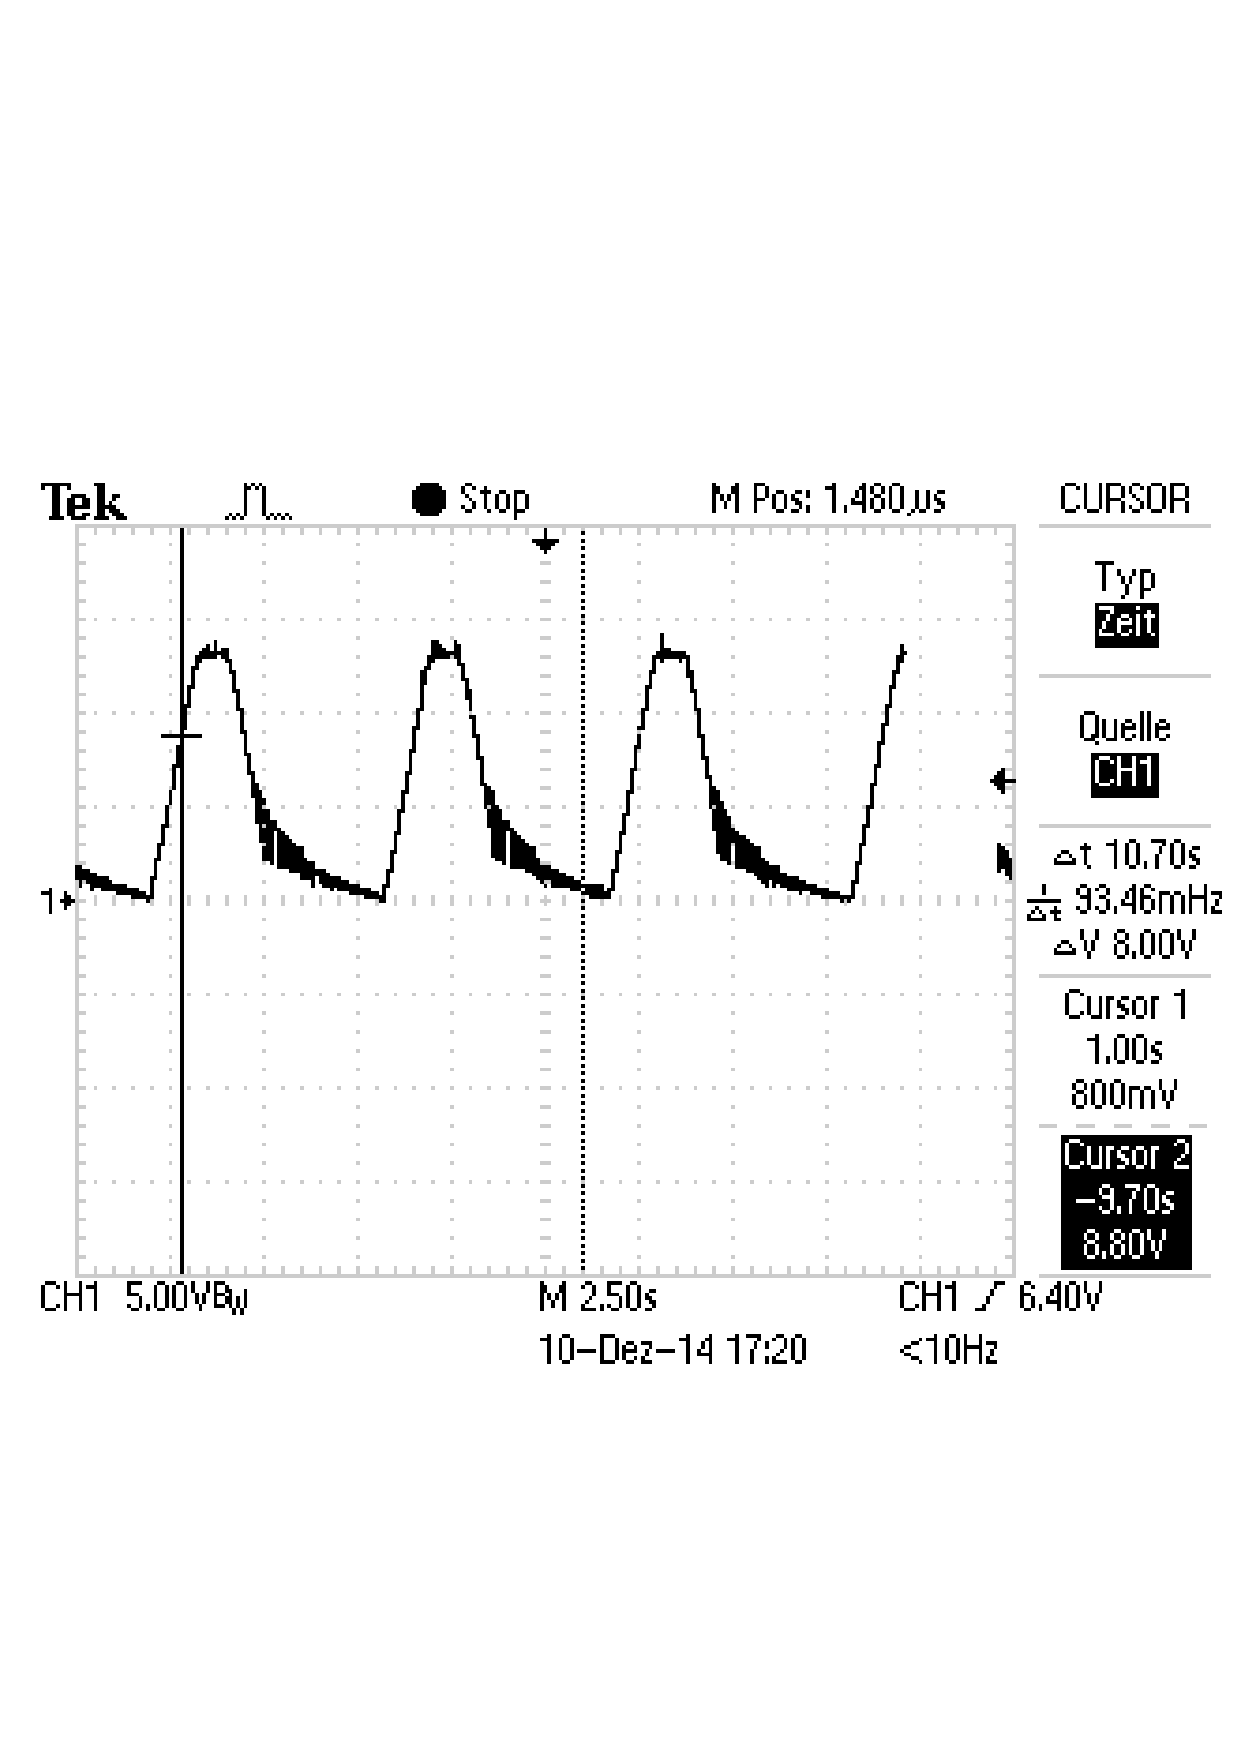
\includegraphics[trim = 0mm 50mm 0mm 50mm, clip, scale = 0.6]{TEK0004.pdf}
  	\caption[Spannugsverlauf beim P-Regler]{Spannugsverlauf beim P-Regler}
  \label{fig:P-Regler_Oszi_3_3_1}
\end{figure}
Da ein Widerstand von \unit[1]{M$\Omega$} verwendet wurde, ist kaum eine Verbesserung aufgrund der Verstärkung zu sehen.

Durch die Änderung der Solltemperatur am Potentiometer setzt die Regelschaltung ein.
\begin{figure}[H]
  \centering
    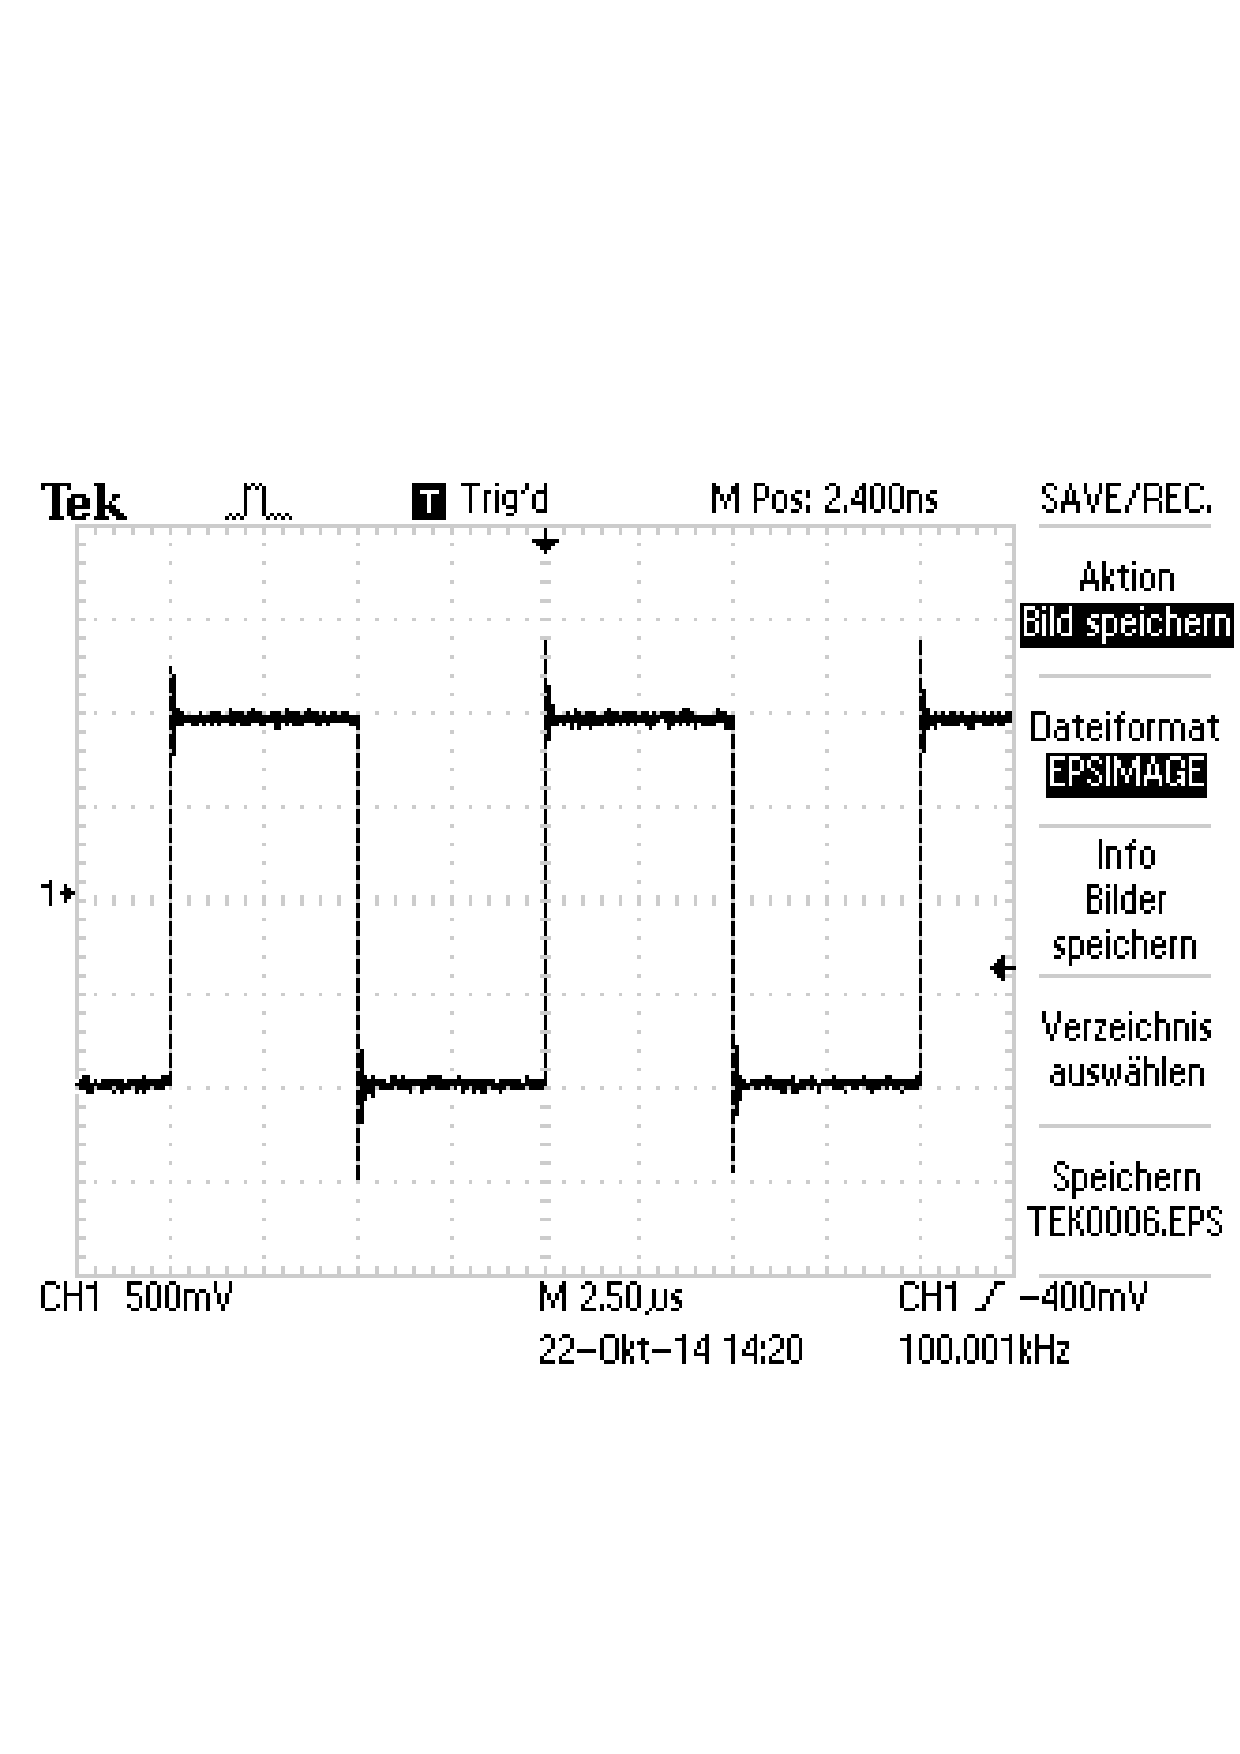
\includegraphics[trim = 0mm 50mm 0mm 50mm, clip, scale = 0.6]{TEK0006.pdf}
  	\caption[Änderung der Solltemperatur P-Regler]{Änderung der Solltemperatur P-Regler}
  \label{fig:P-Regler_Oszi_3_3_2}
\end{figure}
Es ist zu erkennen, dass die Schaltung die Solltemperatur nach kurzer Zeit einstellt, wobei die Schwankung um den Sollwert deutlich zu erkennen ist.

\subsubsection*{Diskussion}
%(immer) die gemessenen werte und die bestimmten werte über die messfehler mit literaturwerten oder untereinander vergleichen
%in welchem fehlerintervall des messwertes liegt der literaturwert oder der vergleichswert?
%wie ist der relative anteil des fehlers am messwert und damit die qualität unserer messung?
%in einem satz erklären, wie gut unser fehler und damit unsere messung ist
%kurz erläutern, wie systematische fehler unsere messung beeinflusst haben könnten
%(wichtig) zum schluss ansprechen, in wie weit die ergebnisse mit der theoretischen vorhersage übereinstimmen
%--------------------------------------------------------------------------------------------
%falls tabellen mit den messwerten zu lang werden, kann die section mit den messwerten auch hinter der diskussion angefügt bzw. eine section mit dem anhang eingefügt werden.
%1-----------------------------------------------1

Die Eigenschaften der Proportionalreglerschaltung konnten in diesem Versuchsteil bestätigt werden, wobei die kontinuierliche Regelung des Ausgangssignals vermutlich mit einem niedrigeren Rückkopplungswiderstand besser gelungen wäre.(kleinerer Verstärkungsfaktor)


\subsection{Proportionalregler mit Integrator}
%kurz das ziel dieses versuchsteiles ansprechen, damit keine zwei überschriften direkt übereinander stehen!
%bei schwierigeren versuchen kann auch der theoretische hintergrund erläutert werden. (mit formeln, herleitungen und erklärungen)

In diesem Versuchsaufbau wird ein Proportionalregler mit Integrator untersucht. Durch den Integrator können Schwingungen der Regelung ausgeglichen werden, zudem ist die Regelwirkung bei einem Verzug der Wirkung stärker.


\begin{framed}
\noindent
Anmerkung: \newline
Der zweite und der dritte Versuchsteil wurden in diesem Versuchsabschnitt vertauscht, da sich dadurch eine bessere Übersicht ergibt.
\end{framed}


\subsubsection*{Verwendete Geräte}
%(immer) eine skizze oder ein foto einfügen, die geräte/materialien !nummerieren! und z.b. eine legende dazu schreiben, besser wäre es das ganze in einem Fließtext gut zu beschreiben.
%falls am anfang des versuches nicht klar ist, was alles verwendet wird, wenn möglich erst am ende ein großes foto von den verwendeten materialien machen!\\

Es werden ein Netzgerät, Widerstände, Kondensatoren, ein Oszilloskop, ein Op-Amp, ein Transistor und ein Lüfter verwendet.


\subsubsection*{Versuchsaufbau}
%skizze zum versuchsaufbau (oder foto) einfügen,   es muss erklärt werden wie das ganze funktioniert und welche speziellen einstellungen verwendet wurden (z.b. welche knöpfe an den geräten für die messung verdreht wurden)

Um dem Proportionalregler einen Integrator hinzuzufügen wird ein Kondensator in Reihe zu Rf geschaltet, C beträgt dabei 100$\mu$F. damit das Signal nicht wegläuft wird ein 100M$\Omega$ Widerstand parallel zu C geschaltet.

\begin{figure}[H] 
  \centering
    \includegraphics[ scale = 0.4]{Auf_2_4.png}
  	\caption[Vereinfachte Schaltskizze des Proportionalreglers mit Integrator]{Vereinfachte Schaltskizze des Proportionalreglers mit Integrator\footnotemark}
  \label{fig:auf_2_4}
\end{figure}
\footnotetext{Abbildungsteile entnommen von http://www.atlas.uni-wuppertal.de/$\sim$kind/ep7\_14.pdf am 06.12.2014}

\subsubsection*{Versuchsdurchführung}
%erklären, !was! wir machen, !warum! wir das machen und mit welchem ziel
%(wichtig) präzize erklären, wie bei dem versuch vorgegangen und was gemacht wurde

Es wird die Schaltung nach Abbildung \ref{fig:auf_2_4} aufgebaut. Zuerst soll die Regelkurve aufgenommen werden. Dafür wird der Lüfter von der Schaltung abgekoppelt (der Stromkreis blieb über Kurzschlussbrücken geschlossen) und das Netzgerät eingeschaltet. Sobald sich der Heizwiderstand auf etwa 70$^\circ$C eingestellt hat, wird der Lüfter wieder angeschlossen und die Temperaturkurve aufgenommen.

Danach soll die Ausgangsspannung mit dem Oszilloskop beobachtet werden. Dafür wird nichts an dem vorherigen Zustand der Schaltung geändert, es wird lediglich die Kurve auf dem Oszilloskop aufgenommen.

Dann wird die Solltemperatur und die Heitzleistung geändert, um zu sehen, ob die Regelschaltung schnell auf die geänderten Werte reagiert. Dafür soll das \unit[10]{k$\Omega$} Potentiometer auf einen neuen Wert eingestellt (ändern der Solltemperatur) und die Betriebsspannung am Netzgerät gesenkt werden. Die Ausgangsspannung wird dann mit dem Oszilloskop aufgenommen.

Im letztem Abschnitt sollen Bauteile des Aufbaus variiert werden und die Ausgangsspannung auf dem Oszilloskop beobachtet werden. Zuerst wird die Spannung am Netzgerät wieder auf den Maximalwert eingestellt. Rf wird durch einen \unit[470]{k$\Omega$} Widerstand ersetzt und das Netzgerät wird angeschaltet. Sobald die Solltemperatur erreicht wird, wird die Ausgangsspannung mit dem Oszilloskop aufgenommen. Dann wird Rf durch einen \unit[470]{k$\Omega$} Widerstand und Ri durch einen \unit[10]{k$\Omega$} Widerstand ersetzt und das Netzgerät eingeschaltet. Sobald die Solltemperatur erreicht wird, wird die Ausgangsspannung mit dem Oszilloskop aufgenommen.

\subsubsection*{Messergebnisse}
%die messwerte in !übersichtlichen! tabellen angegeben
%zu viele kleine tabellen in große tabellen überführen!
%zu große tabellen mit dem [scale]-befehl scalieren oder (falls zu lang) in zwei kleinere tabellen aufteilen
%(wichtig) vor !jeder! tabelle sagen, was gemessen wurde und wie die fehler gewählt wurden und ausreichend !erklären!, !warum! wir unsere fehler grade so gewählt haben

Der Fehler der Zeit wurde mit \unit[0,5]{s} angenommen, da die Zeit von einer Person abgelesen wurde, während die andere Person die Temperatur ablesen musste. Der Fehler der Temperatur wurde mit der Ableseungenauigkeit bestimmt und beträgt \unit[0,1]{$^{\circ}$C}.

\begin{table}[H]
\centering
\begin{tabular}{||r|r||r|r||}

t/s & T/$^\circ$C & t/s & T/$^\circ$C \\ \hline
0 & 70,9 & 75 & 43,0 \\ 
5 & 70,5 & 80 & 42,2 \\ 
10 & 69,0 & 85 & 41,0 \\ 
15 & 66,6 & 90 & 40,5 \\ 
20 & 64,1 & 95 & 40,0 \\ 
25 & 61,3 & 100 & 39,7 \\ 
30 & 59,1 & 105 & 39,6 \\ 
35 & 56,7 & 110 & 39,4 \\ 
40 & 54,3 & 115 & 39,3 \\ 
45 & 52,3 & 120 & 39,2 \\ 
50 & 50,3 & 125 & 39,1 \\ 
55 & 48,4 & 130 & 39,1 \\ 
60 & 47,0 & 135 & 39,1 \\ 
65 & 45,6 & 140 & 39,1 \\ 
70 & 44,4 & 145 & 39,1 \\ 
\end{tabular}
\caption{Messdaten der Regelkurve für die PI-Regler}
\label{tab:3_4}
\end{table}



\subsubsection*{Auswertung}
%zuerst !alle! errechneten werte entweder in ganzen sätzen aufzählen, oder in tabellen (übersichtlicher) dargestellen, sowie auf die verwendeten formeln verweisen (die referenzierung der formel kann in der überschrift stehen)
%kurz erwähnen (vor der tabelle), warum wir das ganze ausrechnen bzw. was wir dort ausrechnen
%danach histogramme und plots erstellen, wobei wenn möglich funktionen durch die plots gelegt werden (zur not können auch splines benutzt werden, was aber angegeben werden muss)
%bei fits immer die funktion und das reduzierte chiquadrat mit angegeben, wobei auf verständlichkeit beim entziffern der zehnerpotenzen geachtet werden muss z.b. f(x)=(wert+-fehler)\cdot10^{irgendeine zahl}\cdot x + (wert+-fehler)\cdot10^{irgendeine zahl}
%bei jedem fit erklären, nach welchem zusammenhang gefittet wurde und warum!
%bei plots darauf achten, dass die achsenbeschriftung (auch die tics) die richtige größe haben und die legende im plot nicht die messwerte verdeckt
%kurz die aufgabenstellung abhandeln
%2-----------------------------------------------2



Im ersten Teil sollte die Regelkurve aufgenommen werden. Bei der Messung ergaben sich die Werte in Tabelle \ref{tab:3_4}, der Plot der Messdaten ist in Abbildung \ref{fig:3_4} zu sehen.

\begin{figure}[H] 
  \centering
    \includegraphics[ scale = 1.5]{3_4.pdf}
  	\caption[Graphische Auswertung der Regelkurve für den PI-Regler]{Graphische Auswertung der Regelkurve für den PI-Regler}
  \label{fig:3_4}
\end{figure}

Dann sollte die Ausgangsspannung mit dem Oszilloskop beobachtet werden. Dabei ergab sich der Verlauf in Abbildung \ref{fig:aus_3_4_1}.


\begin{figure}[H] 
  \centering
    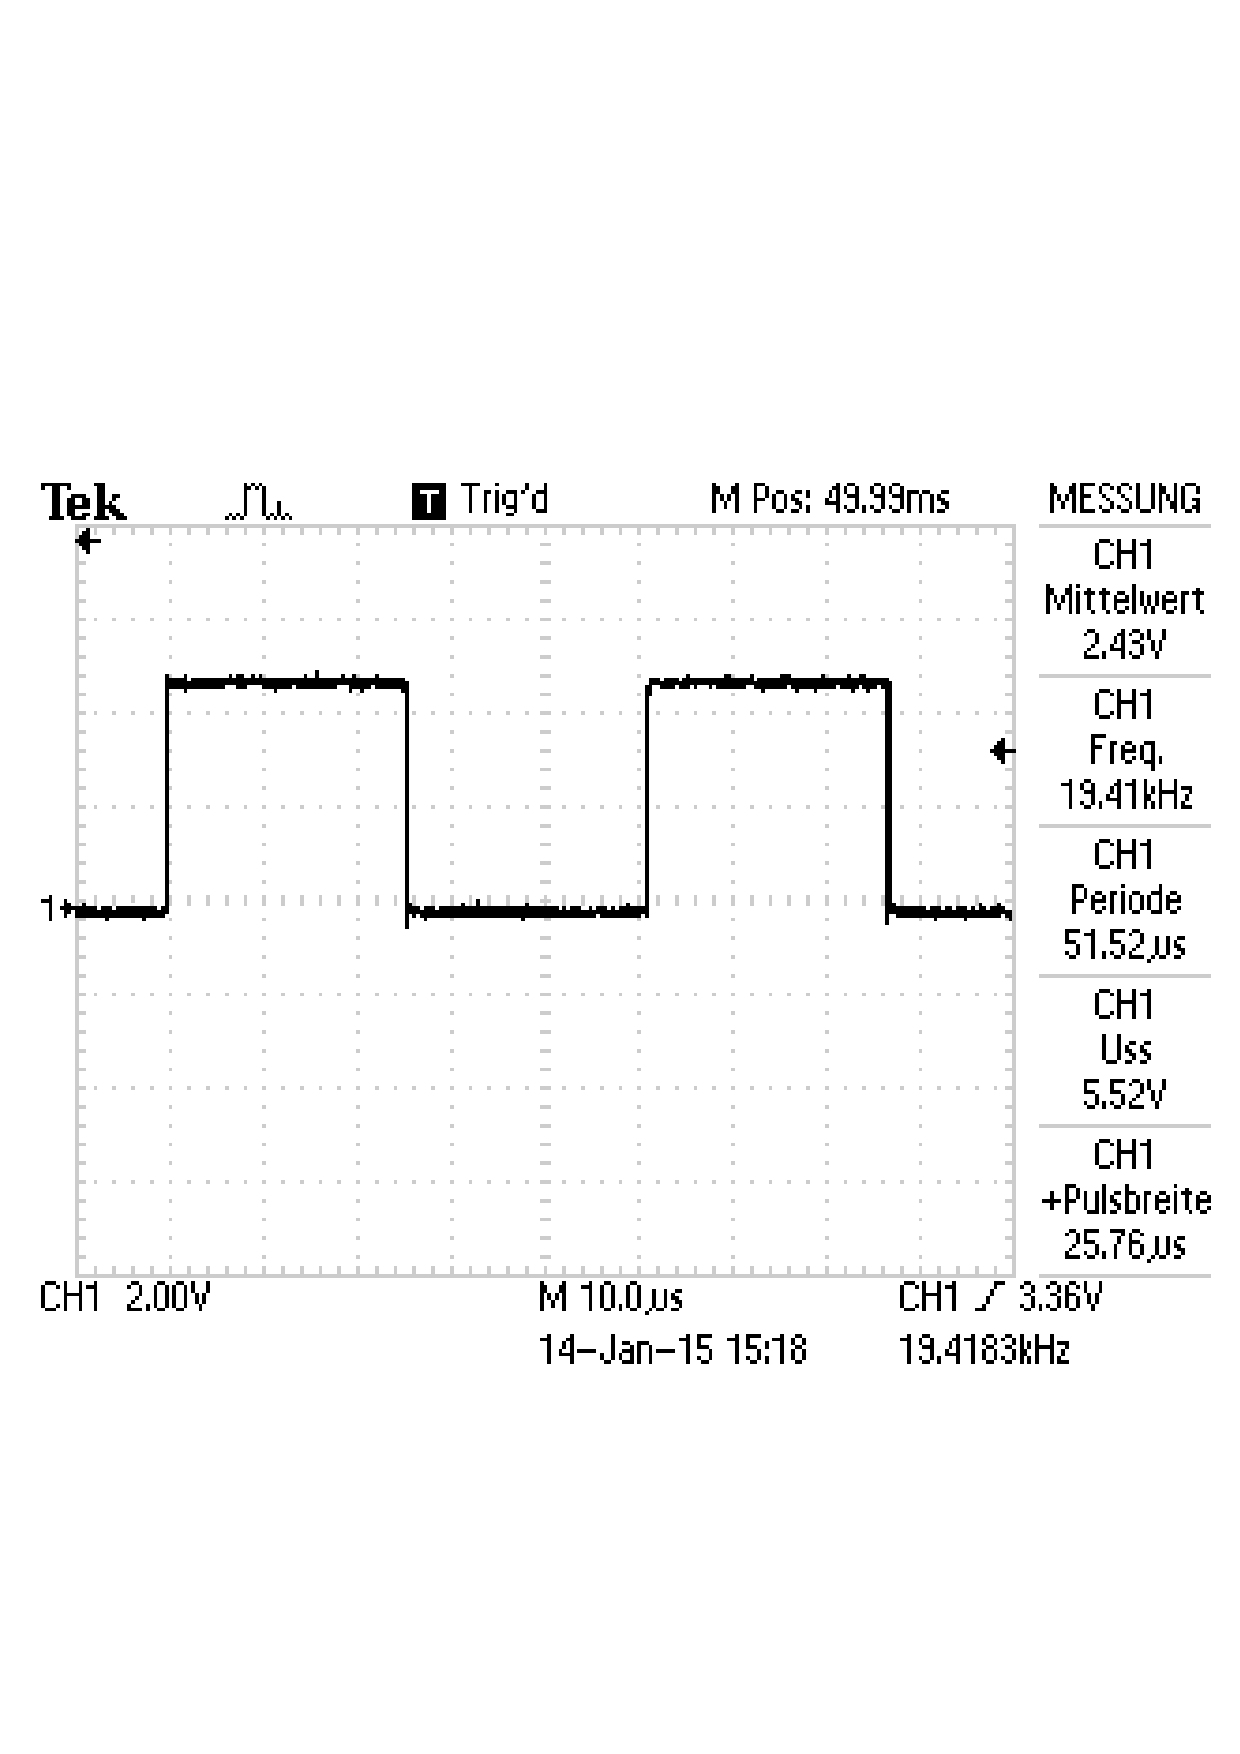
\includegraphics[trim = 0mm 50mm 0mm 50mm, clip, scale = 0.6]{TEK0007.pdf}
  	\caption[Ausgangsspannung in Abhängigkeit der Regelung]{Ausgangsspannung in Abhängigkeit der Regelung}
  \label{fig:aus_3_4_1}
\end{figure}

Im Versuchsteil danach sollte die Solltemperatur und die Heizleistung geändert werden. Der Verlauf der Ausgangsspannung ist in Abbildung \ref{fig:aus_3_4_2} zu sehen.

\begin{figure}[H] 
  \centering
    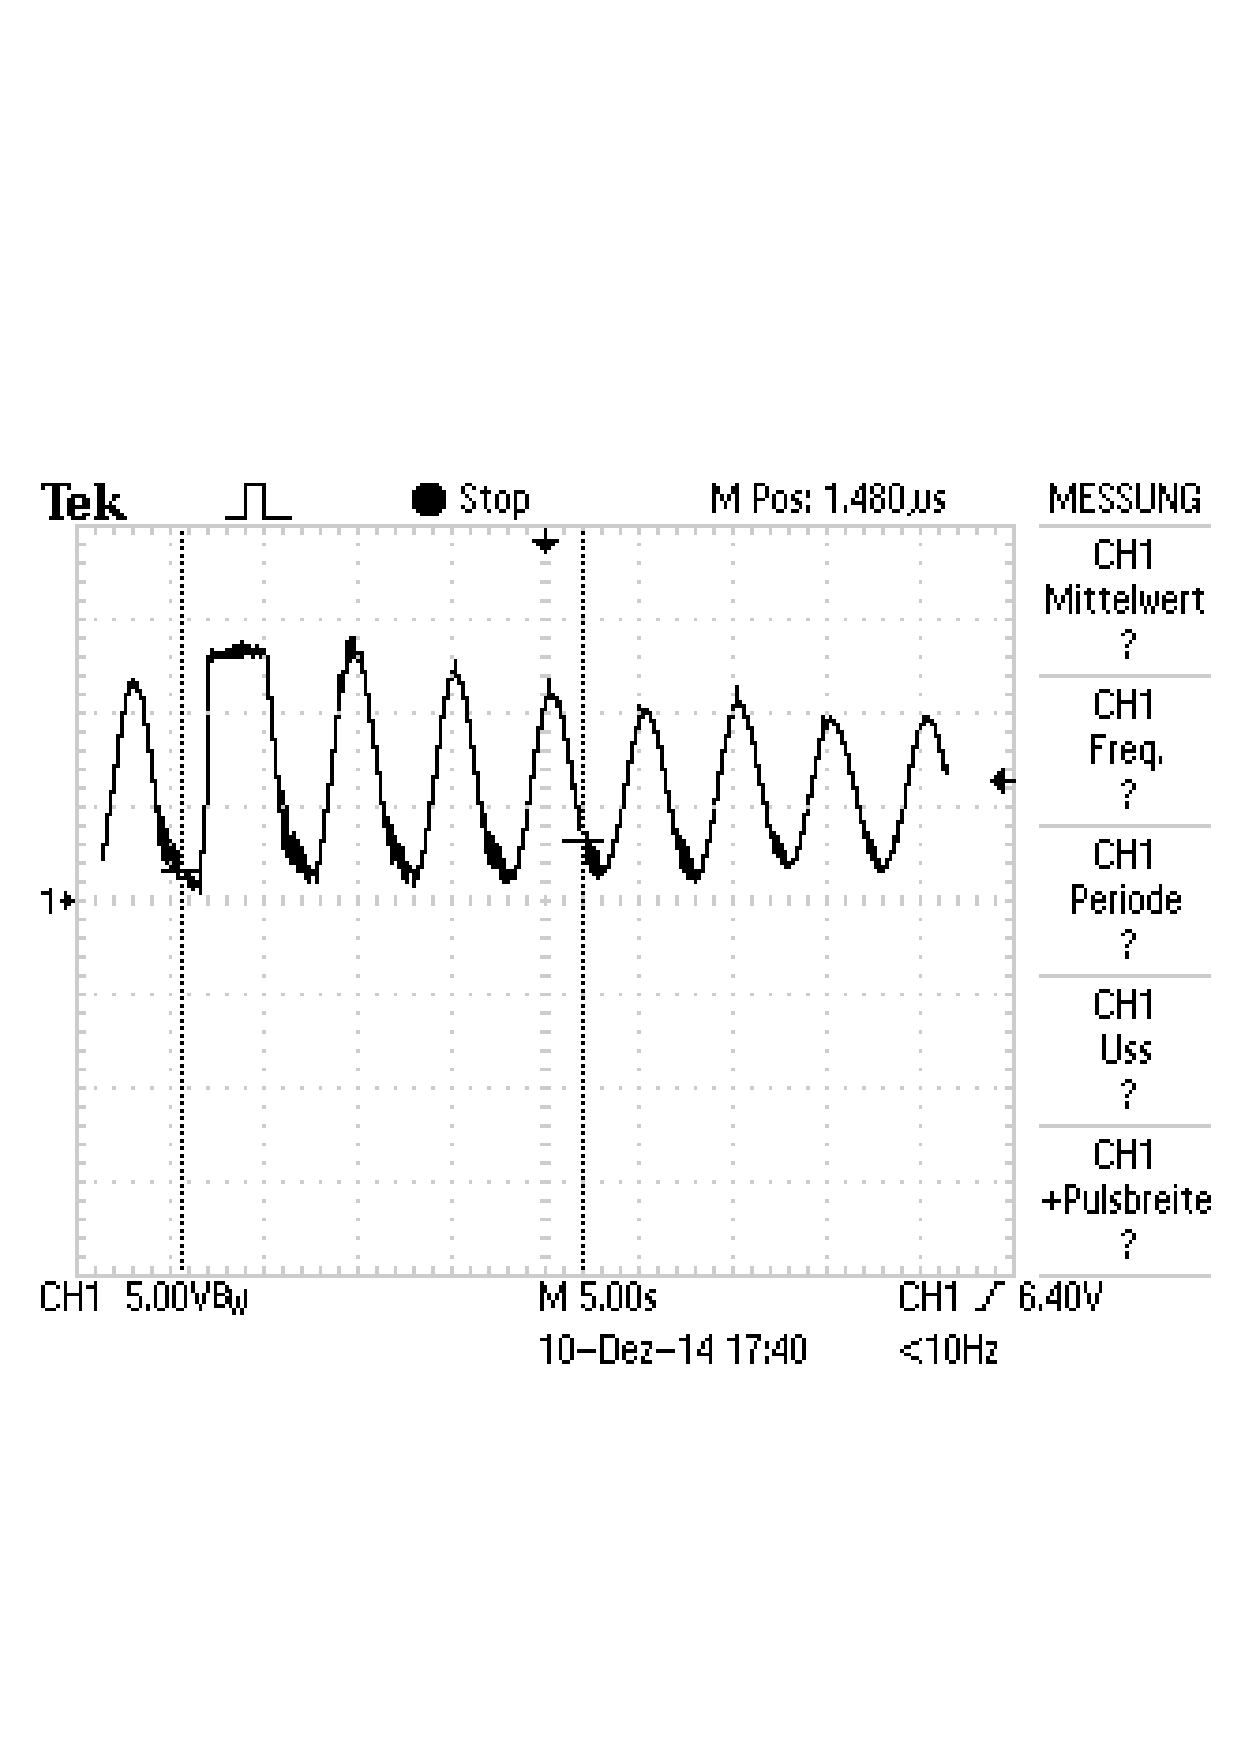
\includegraphics[trim = 0mm 50mm 0mm 50mm, clip, scale = 0.6]{TEK0008.pdf}
  	\caption[Ausgangsspannung in Abhängigkeit der Regelung]{Ausgangsspannung in Abhängigkeit der Regelung}
  \label{fig:aus_3_4_2}
\end{figure}

Im letztem Versuchsteil sollten Bauelemente der Schaltung variiert werden, dafür wurde einmal Rf durch einen 470k$\Omega$ Widerstand ersetzt, die Ausgangsspannung ist in Abbildung \ref{fig:aus_3_4_3} zu sehen.

\begin{figure}[H] 
  \centering
    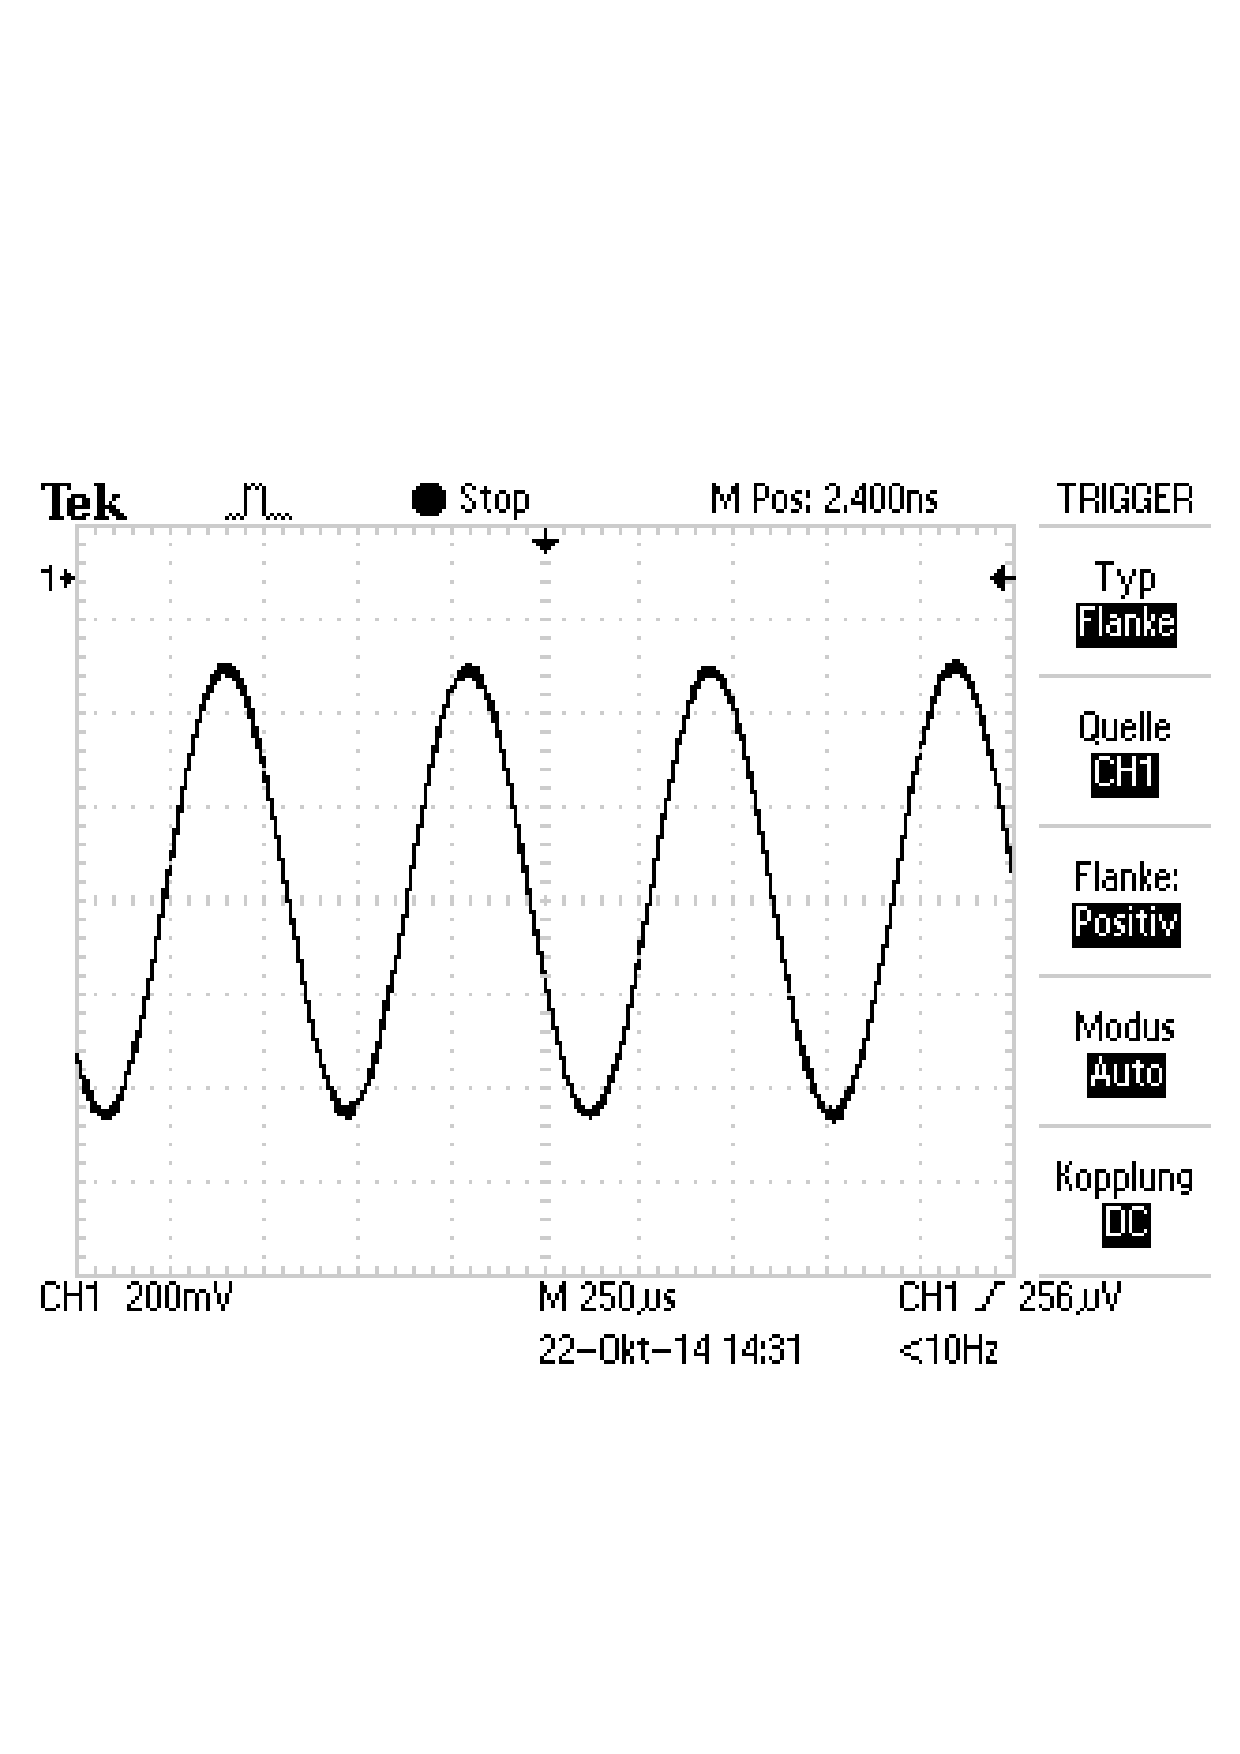
\includegraphics[trim = 0mm 50mm 0mm 50mm, clip, scale = 0.6]{TEK0009.pdf}
  	\caption[Ausgangsspannung in Abhängigkeit der Regelung]{Ausgangsspannung in Abhängigkeit der Regelung}
  \label{fig:aus_3_4_3}
\end{figure}

Dann wurde Rf durch einen \unit[470]{k$\Omega$} Widerstand und Ri durch einen \unit[10]{k$\Omega$} Widerstand ersetzt. Der Verlauf der Ausgangsspannung ist in Abbildung \ref{fig:aus_3_4_4} zu sehen.

\begin{figure}[H] 
  \centering
    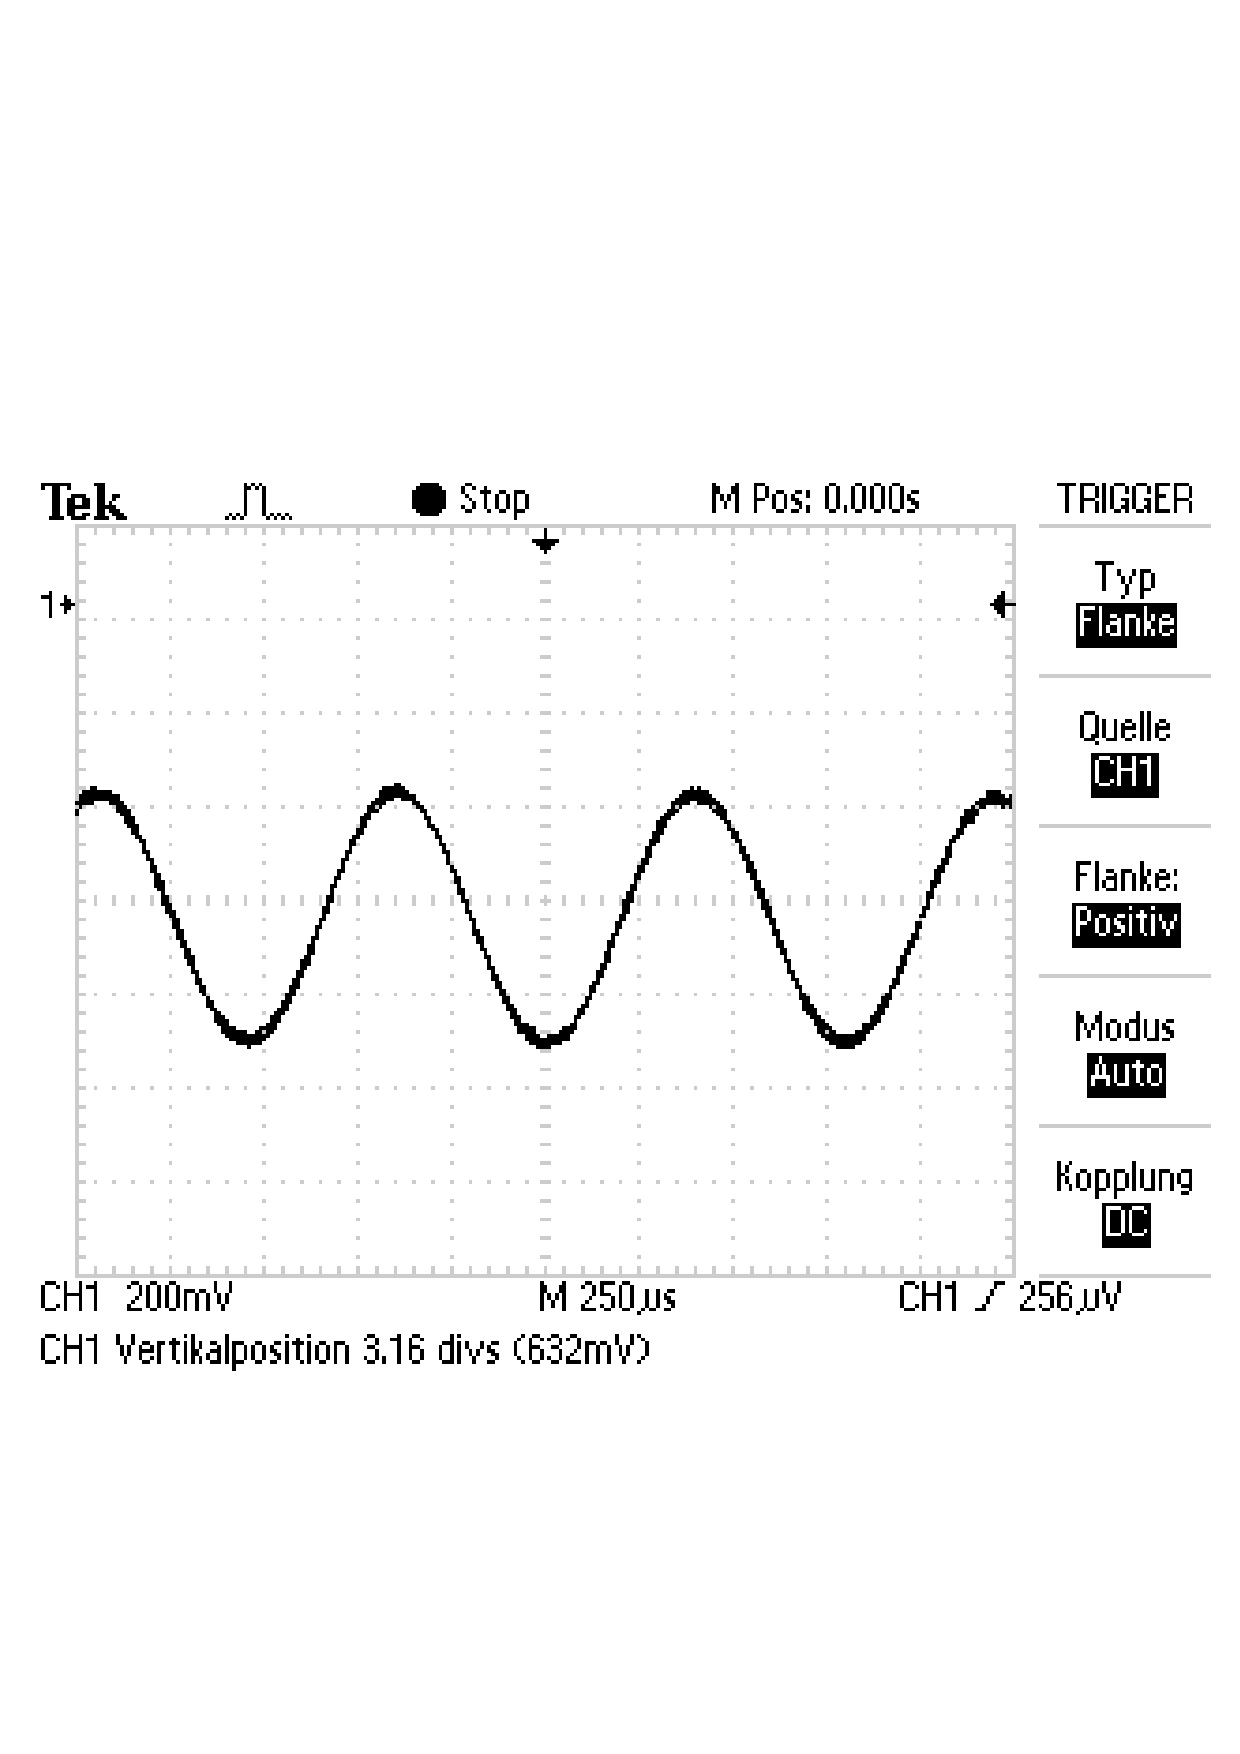
\includegraphics[trim = 0mm 50mm 0mm 50mm, clip, scale = 0.6]{TEK0010.pdf}
  	\caption[Ausgangsspannung in Abhängigkeit der Regelung]{Ausgangsspannung in Abhängigkeit der Regelung}
  \label{fig:aus_3_4_4}
\end{figure}
\subsubsection*{Diskussion}
%(immer) die gemessenen werte und die bestimmten werte über die messfehler mit literaturwerten oder untereinander vergleichen
%in welchem fehlerintervall des messwertes liegt der literaturwert oder der vergleichswert?
%wie ist der relative anteil des fehlers am messwert und damit die qualität unserer messung?
%in einem satz erklären, wie gut unser fehler und damit unsere messung ist
%kurz erläutern, wie systematische fehler unsere messung beeinflusst haben könnten
%(wichtig) zum schluss ansprechen, in wie weit die ergebnisse mit der theoretischen vorhersage übereinstimmen
%--------------------------------------------------------------------------------------------
%falls tabellen mit den messwerten zu lang werden, kann die section mit den messwerten auch hinter der diskussion angefügt bzw. eine section mit dem anhang eingefügt werden.
%1-----------------------------------------------1

Anhand der Regelkurve ist deutlich zu sehen, dass die Schaltung die Solltempatur, sobald sie erreicht wurde, gut hält und keine Schwingung ausführt. Da die Werte für Rf und Ri nicht geändert wurden ist auch hier bei der Aufnahme des Ausgangssignals keine Verbesserung zu erkennen. Beim ändern der Solltemperatur und der Heizleistung ist deutlich zu sehen, wie der Lüfter zu erst mit voller Leistung läuft und sich dann einschwingt. Bei den variierten Bauteilen lässt sich eine deutlich flachere Kurve sehen, dies liegt an den niedrigeren Widerständen, die verwendet wurden. 

\section{Fazit}
%im fazit nochmal alles zusammenfassen und den verlauf der messung abschätzen
%gravierende sytematische probleme bei den messungen nochmal betonen und die wertigkeit unserer ergebnisse einordnen

Bei dem Versuch zeigten alle Schaltungen die erwünschten Regeleigenschaften. Bei der Eichung des NTC hätte ein besseres Ergebnis erzielt werden können, wenn der Aufheizvorgang langsamer durchgeführt worden wäre. Dennoch ist der erwartete exponentielle Verlauf deutlich zu erkennen.

\end{document}

